
% \newcommand{\Suffix}[2]{ {#1}^{\overset{#2}{\leftarrow} } }
% \newcommand{\Suffix}[2]{ {#1}[-{#2}:] }
\newcommand{\Suffix}[2]{ \mathsf{suffix}({#1},{#2})}
\newcommand{\CoinTossingLC}{\Pi_\mathsf{lc}^{\Players(\alpha),k,n}}


\subsection{Blockchain protocols under the longest-chain rule}
Let $\Blockchain$ be an eventual consensus PoS blockchain protocol 
under the longest-chain rule. 
The protocol $\Blockchain$ advances in discrete rounds 
which we call \emph{slots}.
Every participant $u$ in $\Blockchain$ 
maintains a blockchain $\Chain_u$ 
and updates it at every slot using the following simple rule: 
\begin{enumerate}
  \item If a longer blockchain $\Chain$ is available, 
  $u$ sets $\Chain_u \leftarrow \Chain$.

  \item If $u$ is assigned to create a block at this slot, 
  $u$ adds a new block to $\Chain_u$ and broadcasts immediately.
\end{enumerate}

Consider a blockchain $\Chain$ and suppose its most recent block is issued from some slot $s \in \NN$. 
The ``trimmed chain'' $\Chain\TrimSlot{k}$ is defined as 
the blockchain obtained from $\Chain$ by deleting all blocks (from $\Chain$) 
corresponding to the last $k$ slots, i.e., slots $s, s - 1, \ldots, s - k + 1$. 
In addition, we use the expression $\Chain_1 \Prefix \Chain_2$ to mean that 
the chain $\Chain_1$ is a prefix of chain $\Chain_2$. 
Furthermore, given a blockchain $\Chain$ and two slots $t_1$ and $t_2 \geq t_1$, 
$\Chain[t_1 : t_2]$ denotes the chain segment containing all blocks from $\Chain$ 
that are issued from slots $t \in [t_1, t_2]$.

\paragraph{Protocol participants.} 
Let $\Players$ be the set of protocol participants. 
With each party $u \in \Players$ is associated a positive real $\sigma_u \in [0, 1]$ 
so that $\sum_{u \in \Players} \sigma_u = 1$. 
For this analysis, we assume that 
the stakes remain unchanged throughout the execution of the protocol.

\paragraph{The threat and communication model.} 
Let $\alpha \in [0,1]$. 
The adversary can instantly corrupt any player subject to 
a budget $\alpha$: that is, 
at any moment, the set of players $A \subset \Players$ controlled by the adversary 
always satisfy $\sum_{u \in A} \sigma_u \leq \alpha$. 
This adversary is called an \emph{$\alpha$-dominated adversary}. 
If a player is ever corrupted by the adversary, 
he remains under his control for the rest of the protocol. 
The adversary is Byzantine: 
once he controls a player, he can send arbitrary messages on behalf of the player. 
In addition, this is a ``rushing adversary,'' 
i.e., 
he is responsible for delivering messages in an arbitrary order.

Although Praos is designed for a $\Delta$-synchronous network, 
in this analysis we assume a synchronous communication model. 
The results obtained in this setting can be transferred 
to the $\Delta$-synchronous setting via 
the ``$\Delta$-reduction'' technique~\cite{Praos}.



\begin{definition}[Common Prefix property with parameter $k \in \NN$]\label{def:cp}        
    Let $\Chain_1$ and $\Chain_2$ be two blockchains adopted by two honest players 
    at the onset of rounds (i.e., slots) $r_1$ and $r_2$, respectively, with $r_1 \leq r_2$. 
    Then $\Chain_1\TrimSlot{k} \Prefix \Chain_2$. 
\end{definition}
We use the shorthand $\kSlotCP$ for referring to the Common Prefix property defined above. 
Observe that we defined this property in terms of elapsed time, i.e., slots; 
traditionally (cf. \cite{GKL17}), it has been defined in terms of the number of deleted blocks. 


\begin{definition}[Existential Chain Quality property with parameter $s \in \NN$]\label{def:ECQ}        
    Consider slots $t_1, t_2, t$ satisfying $t_1 + s \leq t_2 \leq t$. 
    Let $\Chain$ be the blockchain held by an honest party at slot $t$. 
    Then $\Chain[t_1:t_2]$ contains at least one 
    honestly gneerated block.
\end{definition}
We use the shorthand $\sECQ$ for referring to the ECQ property defined above. 

\smallskip
\begin{definition}[$(\EpsP, k,s)$-secure blockchain protocol]\label{def:blockchain-security}
    Let $\EpsP \in \RR$ and $k, s \in \NN$. 
    A PoS blockchain protocol is $(\EpsP, k, s)$-secure if, 
    except with probability $\EpsP$, 
    it satisfies $\kSlotCP$ and $\sECQ$ properties 
    throughout its execution.
\end{definition}




\subsection{Characteristic strings and leader election}
In Praos and Snow White, 
during each slot, 
each player determine privately and independently 
whether he is a leader for this slot. 
The probability that he succeeds is proportional to his stake. 
Naturally, this means there are empty slots 
which actually help the protocol achieve 
security even with network delay. 
However, since empty slots do not contribute in any blocks, 
we ignore them in our exposition. 
Hence we focus on a leader election process that assigns, 
to each slot, 
a non-empty subset of participants; 
these are the leaders at that slot. 
A leader is eligible to add a block to a 
maximum-length blockchain in his view. 
We can represent the outcome of this leader election scheme 
as a \emph{characteristic string}:


\begin{definition}[Characteristic string]\label{def:char-string}
  A \emph{characteristic string} $w \in \{\A, 1, 2, 3, \ldots \}^*$ 
  corresponds to a particular execution of $\Blockchain$ 
  for each slot $t = 1, 2, \ldots$, 
  $w_t = \A$ if $t$ is assigned to an adversarial participant; and 
  $w_t = k$ if $t$ is assigned to $k$ honest participants, 
  $k \geq 1$.
  By convention, $w_0 = 1$.
\end{definition}

For two characteristic strings $x$ and $w$ on the same alphabet, 
we write $x \Prefix w$ iff $x$ is a strict prefix of $w$. 
Similarly, 
we write $x \PrefixEq w$ iff either $x = w$ or $x \Prefix w$. 
The empty string $\varepsilon$ is a prefix to all strings. 
If $w_t = \A$, we say that ``$\Slot_t$ is adversarial;'' 
otherwise, we say that ``$\Slot_t$ is honest.'' 
Define $\#_\A(w)$ as the number of occurrences of $\A$ in $w$. 
Define $\#_\h(w) \triangleq |w| - \#_\A(w)$.
A slot $t$ is called \emph{$k$-honest} if $w_t = k \in \NN$.
A characteristic string $w$ is called $\Hheavy$ if 
$\#_\h(w) > \#_\A(w)$; 
otherwise, $w$ is called $\Aheavy$. 
We use $w[i : j]$ to denote the substring $w_i w_{i+1}\ldots w_j$.



\paragraph{The distribution $\mathcal{L}(\alpha)$.}
Let $\alpha \in (0, 1/2)$ 
and assume that the adversarial players control an $\alpha$ 
fraction of the stake. 
We consider a leader election mechanism 
which mimics the Praos election except the empty slots. 
Specifically, 
our (idealized) leader election mechanism 
induces 
a distribution $\mathcal{L}_n(\alpha)$ 
on length-$n$ characteristic strings $w = w_1 \ldots w_n$. 
We define $\mathcal{L}_n(\alpha)$ as follows: 
the symbols $w_i$s are independent 
and 
every slot is assigned to at least one slot leader. 
In addition, for all $i$, $\Pr[w_i = \A] = \alpha$.
Furthermore, $\Pr[w_i = j], j \in \NN$ is defined as follows: 
Let $m \in \NN$ be the total number of honest participants. 
Consider the independent Bernoulli random variables $X_i \in \{0, 1\}, i \in [m]$ 
and a tuple $(\sigma_1, \ldots, \sigma_m) \in [0,1]^m$ 
so that $\Pr[X_i = 1] = \sigma_i$ 
and $\sum \sigma_i = 1 - \alpha$. 
Let $H = H_m = \sum_{i =1}^m X_i$. 
Then for $i \in [n]$, 
$$
  \Pr[w_i = j] = (1-\alpha)\cdot
    \frac{\Pr[H = j \mid j \geq 1]}{1 - \Pr[H = 0]}
    \,.
$$

When $n$ is understood from the context, 
we just write $\mathcal{L}(\alpha)$ to denote this distribution.





\subsection{Praos beacon}
Let $\EpsP \in (0,1)$ and $s, k \in \NN$. 
Let $\Blockchain$ be an $(\EpsP, k, s)$-secure eventual consensus PoS blockchain protocol 
under the longest-chain rule, such as 
Ouroboros Praos~\cite{Praos} and Snow White~\cite{SnowWhite}. 



% \subsection{Praos beacon in a synchronous network and no empty slots}


\paragraph{The beacon protocol.}
Let $\kappa$ and let $n$ be a positive integer.\footnote{In this section and the next, 
the symbol $n$ denotes a certain number of rounds. 
However, 
in Section~\ref{sec:intro} and~\ref{sec:model}, 
it denotes the number of participants in a protocol. 
This should not bring confusion since 
the two contexts do not overlap.}
The protocol $\Blockchain$ 
proceeds in epochs $e = 1, 2, \ldots$\,. 
% The length of each epoch is $R \geq n + k$. 
Inside each epoch $e$, 
$\Blockchain$ uses 
an $n$-round 
coin-flipping protocol $\Pi$ 
to generate the \emph{beacon output} $\eta_e$, as follows: 
% which takes a ``seed'' $\eta_{e-1} \UniformIn \{0,1\}^\kappa$ 
% as input and outputs a string $\eta_e \in \{0,1\}^\kappa$, as follows:
\begin{enumerate}
  \item Let $\eta_{e-1}$ be the 
  beacon output from the previous epoch. 
  A uniformly random string $\eta_0 \UniformIn \{0,1\}^\kappa$ is known to all participants at the onset of the first epoch. 

  \item Every new block added during slots $i \in [n]$ contains 
  a uniformly random Boolean string of length $\kappa$; 
  it is called a \emph{nonce}.

  \item Let $u$ be an honest observer at the onset of the next epoch. 
  He computes the beacon output, $\eta_e$, 
  by XORing all nonces recorded in his blockchain 
  along with $\eta_{e-1}$ 
  and then applying a cryptographic hash function to it.
\end{enumerate}
Note that the consistency property of the blockchain 
would ensure that all honestly-held blockchains 
at the onset of epoch $e + 1$ 
will agree about the blocks issued from 
the first $n$ slots of epoch $e$.

Let $L \in \NN$ and suppose that 
the blockchain protocol $\Blockchain$ is $(\EpsP, k, s)$-secure 
inside an epoch. 
Let $R_L$ be the number of ``resets'' 
that the adversary can cause to the beacon, 
i.e., 
the number of candidate values for $\eta_L$ 
is chosen (by the protocol) 
from a set of size $R_L$. 
Then the min-entropy loss 
in the beacon output $\eta_L$ 
is $\log_2(R_L)$. 
We want to show that with high probability, 
this quantity is bounded from above by 
a suitable function. 
The probability in the preceding statement 
depends on 
the randomness in $\eta_0$ and 
the outcomes of the leader election inside the $\Blockchain$, 
i.e., whether a block (and hence its nonce) is emitted by an honest player.


\begin{theorem}[Praos beacon]\label{thm:minentropy-loss-praos}  
  Let $\alpha \in (0, 1/2)$. 
  Suppose Praos 
  remains $(\EpsP, k, s)$-secure 
  inside any epoch 
  whose characteristic string is sampled 
  according to the distribution $\mathcal{L}(\alpha)$.
  Let $\ell$ be the min-entropy loss in 
  the beacon output after $L$ epochs. 
  \begin{itemize}
    \item If $\alpha \leq 0.095$ then 
    $\ell \leq 1/2 \cdot \log_2(1/\EpsP) + \log_2(s) + 0.14 - \alpha$ 
    except with probability $L \cdot (2 \EpsP + s \sqrt{\EpsP} )$.

    \item Otherwise, there is a positive constant $c = c(\alpha, s)$ so that 
    $\ell \leq 1/2 \cdot \log_2(1/\EpsP) 
    + c \alpha s
    % + s/2 \cdot \log_2(1+3\alpha)
    $ 
    except with probability $L \cdot (2 \EpsP + (1.1 - 0.8 \alpha) s (1+3\alpha)^s \sqrt{\EpsP} )$. 
    We can take $c = 3$ for $\alpha \geq 1/3$ and $s \geq 4$.
  \end{itemize}
\end{theorem}

The proof of Theorem~\ref{thm:minentropy-loss-praos} 
is presented in Section~\ref{sec:proof-praos-theorem}. 

\begin{remark*}
  If $0.095 < \alpha < 1/3$, we can obtain tighter upper bounds on both $\ell$ and the bad probability 
  by using relevant upper bounds from~\eqref{eq:grindign-praos-second-moment} 
  in the proof of Theorem~\ref{thm:minentropy-loss-praos}. 
  The $\log_2(1/\EpsP)$ term in the min-entropy loss $\ell$ 
  is inevitable if we want 
  the bad probability to be at most $\EpsP^\delta$ 
  for some positive real constant $\delta \in (0, 1)$. 
  The factor $1/2$ in front of the $\log_2(1/\EpsP)$ term 
  is an artifact of the tail bound using the second-moment method.
  Finally, when $\alpha \geq 0.1$, 
  both the number of adversarial resets $R_L$
  and the bad probability 
  grow exponentially in $s$.
\end{remark*}


% The goal of this section is to derive positive reals $\EpsP \in (0, 1)$ and $\rho \in (0, \kappa)$ 
% so that the protocol $\Pi$ is $(\EpsP, \rho)$-secure. 
% Specifically, we have the following: 
% Let 
% \begin{align}
%     % \qquad\text{and}\qquad
%     % \beta &= \\
%   \rho &= \log_2 n 
%     % + \tau/2 
%     + \frac{\log_2(1/\EpsP)}{2}
%     +  
%     \begin{cases}
%       % 0.43 (1 - 2\alpha)
%       %     \,, &\quad\text{if}\quad\epsilon \in (0, 1/3]\,, \\
%       % 0.24 (1 - 2\alpha) (5/2 - 3 \alpha)
%       % % 15/16 - 0.24 \epsilon(1+\epsilon)(1-\epsilon/2)
%       %     \,, &\quad\text{if}\quad\epsilon \in (1/3,0.809]\,, \\
%       % 2/3
%       %     \,,&\quad\text{otherwise}\,.
%       0
%           \,, &\quad\text{if}\quad\alpha \in (0, 0.0955)\,, \\
%       n \cdot (0.067 + 1.92 \alpha - 1.44 \alpha^2)
%           \,, &\quad\text{if}\quad\alpha \in [0.0955, 1/3)\,, \\
%       n \cdot (0.237 + 0.86 \alpha)
%           \,, &\quad\text{if}\quad\alpha \in [1/3, 1/2)\,.
%     \end{cases}    
%   % \,.
% \end{align}


% The theorem above is an easy corollary 
% of Theorem~\ref{thm:praos-tail-gamma} 
% if we use $\epsilon = (1 - 2\alpha)/2$ 
% and $\EpsG = \log_2(1/\EpsP)$ in that theorem statement.

% \begin{remark}
% In Section~\ref{sec:coin-tossing}, 
% we develop coin-flipping protocols (with an integer parameter $d$) 
% where we can effectively ``slow down'' the growth of $\rho$ by a factor $1/d$.
% Specifically, 
% in those protocols, nonces are associated with slots.
% the min-entropy loss in those protocols 
% depends linearly on $k/d$ 
% but logarithmically on $n/d$; 
% hence we can avoid a loss in $\rho$ 
% by suitably increasing the failure probability.
% It is not obvious how to do the same for protocol $\Pi$, however, 
% as nonces are associated with blocks, not slots. 
% \end{remark}


\iftoggle{drawfigs}{

\begin{figure}
  \centering
  \pgfmathsetmacro{\k}{100}
  \pgfmathsetmacro{\d}{1}
  \pgfmathsetmacro{\T}{24 * \k}
  \pgfmathsetmacro{\tau}{30}
  \pgfmathsetmacro{\n}{(\T - \k)/\d}
  \pgfmathsetmacro{\ell}{\k/\d}
  \pgfmathsetmacro{\ellPlusN}{\ell + \n}
  \begin{tikzpicture}[trim axis left,
    declare function={rho_praos_small_alpha(\a) = log2(\n + \ell) + \tau / 2 ; 
      rho_praos_mid_alpha(\a) = log2(\n + \ell) + \tau / 2 + \n * (0.067 + 1.92*\a - 1.44 * \a * \a) ; 
      rho_praos_large_alpha(\a) = log2(\n + \ell) + \tau / 2 + \n * (0.237 + 0.86 * \a); 
      rho_geom_small_alpha(\a) = 2 * log2(\n) + \tau/2 + \ell * log2( sqrt(1 + \a)/(1 - \a) );
      rho_geom_large_alpha(\a) = 2 * log2(\n) + (\tau + \ell * log2( 1/\a ) )/(2 - (3 * \a - 1)/(2 * \a * \a));
    }
    %    declare function = { entropy(\x) = 1; },
    ]
    \begin{axis}[domain=0:0.5,
      samples=100,
      enlarge x limits=false,
      grid=both,
      no markers,
      x label style={at={(axis description cs:0.5,-0.1)},anchor=north},
      y label style={at={(axis description cs:-0.1,.5)},anchor=south},
      xlabel={$\alpha$, relative adversarial stake},
      ylabel={$\rho$, loss in min-entropy (bits)},
      % there is one default value for the `legend pos' that is outside the axis
      legend pos=outer north east,
      % (so the legend looks a bit better)
      legend cell align=left
      ]
      \addplot +[thick,domain=0:(0.0955),red,forget plot] plot (\x, {rho_praos_small_alpha(\x)});
      \addplot +[thick,domain=0.0955:(1/3),red,forget plot] plot (\x, {rho_praos_mid_alpha(\x)});
      \addplot +[thick,domain=(1/3):(0.5),red,legend] plot (\x, {rho_praos_large_alpha(\x)});
      \addlegendentry{Praos, $\ellPlusN$ rounds}

      \addplot +[thick,domain=0:(1/3),blue,forget plot] plot (\x, {rho_geom_small_alpha(\x)});
      \addplot +[thick,domain=(1/3):(1/2),blue,legend] plot (\x, {rho_geom_large_alpha(\x)});
      \addlegendentry{$(\ell, \n, \alpha)$-geometric game, $d = 1$}
    \end{axis}
  \end{tikzpicture}
  \caption{Min-entropy loss in Praos (red) and in the $(\ell, n, \alpha)$-geometric game (blue).}
  \label{fig:rho-praos}
\end{figure}

} % end iftoggle{drawfigs}


% As we discussed after Definition~\ref{def:coin-flipping-security}, 
% the adversarial participants in an $(\EpsP, \rho)$-secure 
% coin-flipping protocol $\Pi$ can choose the output $\eta$ 
% from a set $X$ of size $2^\rho$. 
% As $\Pi$ is conducted on the blockchain protocol $\Blockchain$, 
% the elements of $X$ are determined by 
% the set $C$ of all possible maximally long blockchains 
% at (or after) slot $n + k$. 
% Due the the $\kSlotCP$ property of $\Blockchain$, 
% these chains contain the same blocks corresponding to slots $1, \ldots, n$. 
% It follows that $\rho = \log_2 |X| = \log_2 g$.
% We call $g$ the \emph{grinding power} of the adversary. 





\subsection{Forks, viable blockchains, and grinding power}

% \paragraph{Blockchain execution as a ``fork.''} 
Consider an abstract execution of $\Blockchain$ 
corresponding to the characteristic string $w$ 
where 
all blockchains are arranged in a rooted tree; 
this tree is called a \emph{fork}. 
If a block $B$ is issued from slot $t$, 
we say that $B$ has label $t$.
Two blockchains $\Chain_1, \Chain_2$ in a fork $F$ are considered ``different'' 
if and only if there is a slot from which 
$\Chain_1$ contains a block but $\Chain_2$ does not. 
A blockchain $\Chain \in F$ is called \emph{viable} (or \emph{competitive}) 
if the length of $\Chain$, denoted by $|\Chain|$, 
is at least $\#_\h(w)$. 
The rationale is that an honest blockchain $\Chain$ is broadcast immediately 
and hence any blockchain adopted by a future honest leader
must be at least as long as $\Chain$. 
% In addition, if an honest participant is presented with 
% a blockchain $\Chain$ with length at least $\#_\h(w)$, 
% that participant would possibly prefer $\Chain$ 
% over a blockchain containing only honestly-emitted blocks 
If an honest observer (or leader) has to choose from multiple viable blockchains for adoption, 
we assume that the tie is broken by the adversary. 

Considering any fork $F$ and an honest blockchain $\Chain$ in $F$, 
a \emph{viable adversarial extension of $\Chain$} 
is an adversarial blockchain $\Chain' \in F$ 
such that $\Chain \Prefix \Chain'$, 
$\Chain'$ has the maximum length in $F$, 
and, importantly, $\Chain'$ contains only adversarial blocks after the prefix $\Chain$. 
Note that every adversarial extension 
viable at the onset of slot $n + 1$, 
corresponds to a choice 
for the output of the coin-flipping protocol. 
Each of these extensions contains a last honest block as its prefix. 
Thus we focus on upper bounding, 
over all forks for a given characteristic string, 
the total number of viable adversarial extensions 
of the honest blocks.
Note that a prerequisite to creating an adversarial extension 
of an honest block with label $h$ is that 
the suffix $w[h + 1 : n]$ must be $\Aheavy$.
We formalize this notion in the definition below.

\begin{definition}[Option Sequences and Grinding Power]\label{def:option-sequence}
  Let $w$ be a characteristic string of length $n$. 
  We say that a sequence
  $
    0 \leq i_0 < i_1 < \cdots < i_k \leq n
  $
  is an \emph{option sequence} if
  \InlineCases{
    \item $i_0 = 0$ or 
    % $w_{i_0} = \h$, 
    $i_0 \neq \A$, 
    \item $w_{i_j} = \A$ for each $j > 0$, and
    \item $k \geq \#_\h(w[i_0 +1 : n])$.
  }
  We define the \emph{grinding power} of $w$, denoted $g(w)$, 
  as the 
  number of distinct option sequences for $w$.
\end{definition}

% Let $\Suffix{w}{d}$ denote the length-$d$ suffix of a string $w$.

% Fix a characteristic string $w$ of length $n$.
%  and 
% let $x = \Suffix{w}{d}$. 
% Condition on the event that $\#_\h(x) = z$.
% The grinding power of $x$, which we denote by $g\left( x \Given \wt(x) = d - z  \right)$, 
% equals the number of distinct option sequences corresponding to $x$ 
% defined as
Let $w = xy$ be a characteristic string. 
Then
\begin{equation}\label{eq:S_y}
    % S(d, z) 
    % \defeq \sum_{i \geq z}^{d - z}{ \binom{d - z}{i} } 
    S(y) 
    \defeq \sum_{i \geq \#_\h(y)}^{\#_\A(y)}{ \binom{\#_\A(y)}{i} } 
    % \,.
\end{equation}
is the number of viable blockchains $\Chain$
in an execution on $w$ 
so that the last honest block in $\Chain$ occurs in slot $|x|$. 
By summing over all honest slots, 
the total number of viable blockchains for $w$ is 
\begin{equation}\label{eq:g_praos}
    g(w) 
    % = \sum_{d=1}^n g(\Suffix{w}{d})
    = \sum_{\substack{
        x,y : w = xy, \\ 
        |x| \geq 0, \text{and}\\ 
        \text{slot $|x|$ is honest} }
      } w_{|x|}\, S(y)
    \,.  
\end{equation}




\subsection{A tail bound on $g$ from its second moment}
Let $\epsilon \in (0, 1)$ and write $\alpha = (1 - \epsilon)/2$, and 
think of $\epsilon$ as the ``adversarial bias.'' 
Let $W \sim \mathcal{L}_n(\alpha)$ and 
Define 
\begin{align}\label{eq:suffix-prob-binomial}
    B_{n, \epsilon}(k) 
    &= \Pr[ \#_\A(W_1 \ldots W_n) = k ]  
    = 2^{-n}\binom{n}{k} (1-\epsilon)^k (1 + \epsilon)^{n-k} 
    =  \binom{n}{k} 
        \left(\frac{1-\epsilon}{2}\right)^n 
        \left(\frac{1 + \epsilon}{1-\epsilon} \right)^{n-k} 
        \,.
\end{align}
% Define
% \begin{equation}\label{eq:prob-Hheavy}
%   h(n) 
%   \triangleq \Pr[\text{$W$ is $\Hheavy \mid W$ has length $n$}] 
%   = \sum_{k \geq n/2} B_{n, \epsilon}(k)
%   \,.
% \end{equation}
For the sake of convenience, 
we overload the function $S(\cdot)$ 
to count the number of characteristic strings, 
of length $d$, containing $z$ honest indices.
\begin{equation}\label{eq:S_d_z}
  S(d, z) 
    \defeq \sum_{i \geq z}^{d-z}{ \binom{d-z}{i} } 
    \quad\text{and}\quad
  S(d) \defeq \sum_{z = 0}^{d/2} S(d,z)
  \,.  
\end{equation}

Recall that for any characteristic string $w = w_1 w_2 \ldots$, 
we have $w_0 = 1$ by convention. 
Let $\lambda$ be a positive real, $\lambda \geq 1$. 
% (For our application, we would only use $\lamba = 2$.)
We can express the $\lambda$th moment of the grinding power as
\begin{align}\label{eq:grinding-power-moment-praos}
    \Exp\, g(W)^\lambda 
    &= \sum_{t = 0}^n \Pr[W_t \neq \A] \cdot \Exp (W_t\, S(W_{t+1}\ldots W_n))^\lambda \nonumber \\
    &= \sum_{t = 0}^n
    \sum_{k \geq 1} 
      \Pr[W_{t} = k] \Pr[\text{$W_{t+1}\ldots W_n$ is $\Aheavy$}]\cdot (k S(n - t) )^\lambda \nonumber \\
    &= A(\epsilon, \lambda) 
      \sum_{t = 0}^n 
      \Pr[\text{$W_{t+1}\ldots W_n$ is $\Aheavy$}]\cdot S(n-t)^\lambda \nonumber \\
    &=  %\Pr[\text{$W_1$ is honest}]\,
        A(\epsilon, \lambda)
        \cdot 
        \sum_{d=1}^n \sum_{z = 0}^{ d/2 } B_{d, \epsilon}(d - z) S(d,z)^\lambda
\end{align}
where 
\begin{equation}
  A(\epsilon, \lambda) \defeq \sum_{k\geq 1} \Pr[W_1 = k] \cdot k^\lambda
  % \,,
  \label{eq:A}
\end{equation}
and, by convention, 
the inner sum in~\eqref{eq:grinding-power-moment-praos} 
runs for $z = 0, 1, \ldots, \lfloor d/2 \rfloor$.

The first equality in the derivation of~\eqref{eq:grinding-power-moment-praos} follows from 
% the subadditivity of the convex function 
% $x \mapsto x^\lambda$ for $\lambda \geq 1, x \geq 0$,  
~\eqref{eq:g_praos}. 
The second equality follows 
since only $\Aheavy$ suffixes of $w$ contribute to $g(w)$ 
and that the symbols in $W$ are independent. 
The third equality follows from rearranging the sums. 
The last equality follows from~\eqref{eq:suffix-prob-binomial} 
and~\eqref{eq:S_d_z}.

Our goal \footnote{
It turns out that the the second moment of $g(W)$ grows 
much faster than its first moment. In fact, 
Chebyshev's inequality on $g(W)$ fares only marginally better 
than what we get via Markov's inequality on $g(W)^2$. 
% Thus we defer the analysis of the first moment in 
% % Appendix~\ref{app:grinding-praos}.
% the full version~\cite{GrindingFullVersion}.
}
is to develop a tight upper bound on $\Exp g(W)^2$ 
which, when used in Markov's inequality, 
would give us a tail bound on $g(W)$. 

\begin{lemma}[Tail bound on $g$]\label{lemma:praos-tail-gamma}
  Let $\epsilon, \EpsP \in (0, 1)$ and $n, k, s \in \NN$. 
  Let $W \sim \mathcal{L}_n((1-\epsilon)/2)$.
  % Let $m(W)$ denote the right-hand side of~\eqref{eq:grinding-praos-second-moment}. 
  Let $E$ be the event that 
  $\Blockchain$ remains $(\EpsP, k, s)$-secure during 
  the $n$ slots represented by $W$. 
  Let $m(W)$ be an upper bound on $\Exp[ g(W)^2 \mid E]$.
  Let $\gamma = (m(W)/\EpsP)^{1/2}$.
  Then 
  $
      \Pr\left[g(W) \geq \gamma\right] \leq 2 \EpsP
      % \,.
  $.
\end{lemma}
\begin{proof}
  % Recall the event $E$ defined in Lemma~\ref{lemma:grinding-praos-second-moment}.
  Let $\gamma \in \NN$. 
  Since $g(W)$ is non-negative, 
  $$
    % p_\gamma 
    \Pr[g(W) \geq \gamma]
    \leq (1 - \Pr[E]) + \Pr[g(W)^2 \geq \gamma^2 \mid E] 
    \leq \EpsP + m(W)/\gamma^2
  $$ 
  by Markov's inequality on the non-negative random variable $g(W)^2$. 
  We set $\gamma$ to be large enough so that the above quantity is at most $2 \EpsP$. 
  Equivalently, 
  $m(W)/\gamma^2$ would be at most $\EpsP$, 
  or $\gamma$ is at least $\sqrt{m(W)/\EpsP}$. 
\end{proof}


\subsection{The second moment of $g$}

We begin by stating three helpful claims 
whose proofs will be presented later.

\begin{claim}\label{claim:multiple-honest-blocks}
  For $\epsilon \in (0, 1)$, 
  $
    A(\epsilon, 2) 
    % \leq 
    % \frac{(1 + \epsilon)^2 (5 + \epsilon)}{16 \left( 1 - e^{(1 + \epsilon)/2} \right)}
    % \leq 2^{- 0.3 + 1.85 \epsilon}
    % \leq 2^{- 1.3 + 0.41 \epsilon}
    % \leq 1
    \leq 0.8 (1 + 2 \epsilon)
    \,.
  $
\end{claim}


% $\Exp H_m^2 \leq \Exp \GeomOneMinusAlpha^2 = (2 - \alpha)/\alpha^2$. 
% The last equality is a known fact; see~\eqref{eq:geom-moments-1-2} 
% which gives the second moment of $\GeomAlpha$. 
% Therefore,
% \begin{align}
%   \sum_{k\geq 1} \Pr[W_1 = k]\, k^\lambda 
%   &\leq \frac{1 - \alpha}{1 - e^{-(1 - \alpha)}} \frac{2 - \alpha}{\alpha^2} \nonumber \\
%   % &= \frac{1+\epsilon}{2} \frac{3 + \epsilon}{2} \frac{4}{(1 - \epsilon)^2}
%   &= \frac{(1+\epsilon)(3 + \epsilon)}{(1 - \epsilon)^2\left( 1 - e^{-(1 + \epsilon)/2} \right)}
%   \,.
% \end{align}



\begin{claim}\label{claim:t1star-variance-exact}
  Let $\epsilon \in (0,1)$ and 
  let $d,z$ be non-negative integers where $d \geq 2$ and $z \leq d/3$. 
  \begin{align*}
    B_{d, \epsilon}(d-z) S(d,z)^2
    &\leq \begin{dcases} 
    \left( (5-3 \epsilon)/2 \right)^d \,,
        &\quad \text{if}\quad
        0 < \epsilon < 1/3 \,, \\
    \left( 2^{2/3} \phi(\epsilon) \right)^d \,,
    %\frac{6}{\sqrt{5 d}}
        &\quad \text{if}\quad
        1/3 \leq \epsilon < 1 \, ,
    \end{dcases}
  \end{align*}
  where
  \begin{align}
    \phi(\epsilon) 
    &\triangleq \frac{3}{2} (1+\epsilon)^{1/3} (1-\epsilon)^{2/3}\label{eq:phi_eps} 
    \,.
  \end{align}
\end{claim}

\begin{claim}\label{claim:t2star-variance-exact}
  Let $\epsilon \in (0,1)$ and 
  let $d,z$ be non-negative integers where $d/3 \leq z \leq d/2$. 
  \begin{align*}
    B_{d, \epsilon}(d-z) S(d,z)^2
    &\leq \begin{cases} 
    \left( 2^{2/3} \phi(\epsilon) \right)^d \,,
        &\quad\text{if}\quad 0 < \epsilon \leq 0.6\,, \\
    \left( (5/3) \phi(\epsilon)  \right)^d \,,
        &\quad\text{if}\quad 0.6\leq \epsilon < 0.81\,, \\
    1 \,,
        &\quad\text{if}\quad 0.81 \leq \epsilon < 1
        \,.
    \end{cases}
  \end{align*}
\end{claim}
% We defer the proofs of these claims in the next subsection .


% \subsection{Moment-bounds on the grinding power}

% \begin{lemma}[First moment of the grinding power]\label{lemma:grinding-power-mean}
% Let $W \sim \Binomial(n, (1-\epsilon)/2)$ for $\epsilon \in (0,1)$. 
% Then
% \begin{align*}
%     \phi(\epsilon)^n/4 \leq \Exp g(W) \leq n\, \gamma(\epsilon)^n
%     \,,\qquad\text{if}\quad \epsilon < 0.6\,, \\
%     \ln(n)/2 \leq \Exp g(W) \leq n
%     \,,\qquad\text{if}\quad \epsilon \geq 0.6\,,
% \end{align*}
% where
% \begin{align}
%     \gamma(\epsilon) 
%     &\defeq (1-\epsilon)/2 + \sqrt{1-\epsilon^2} \label{eq:gamma_eps}
%     \,.
% \end{align}

% \end{lemma}


\begin{lemma}[Second moment of $g$]\label{lemma:grinding-praos-second-moment}
  Let $\epsilon, \EpsP \in (0, 1)$ and $n, k, s \in \NN$. 
  Let $W \sim \mathcal{L}_n((1 - \epsilon)/2)$. 
  Let $E$ denote the event that 
  the blockchain protocol $\Blockchain$ 
  remains $(\EpsP, k, s)$-secure throughout 
  the $n$ slots represented by $W$. 
  Then
  \begin{equation}\label{eq:grindign-praos-second-moment}
    \Exp[ g(W)^2 \mid E] 
    \leq 
      % s^2/2 
      % s^2 
      % 2^{- 1.3 + 1.85 \epsilon} 
      % A(\epsilon,2)
      0.4 s^2 (1 + 2\epsilon)
      \cdot \begin{cases}
      \left( (5-3 \epsilon)/2 \right)^s & \text{if}\quad 0 < \epsilon \leq 1/3\,, \\
      \left( 2^{2/3} \phi(\epsilon) \right)^s & \text{if}\quad 1/3 < \epsilon \leq 3/5\,, \\
      \left( (5/3) \phi(\epsilon) \right)^s & \text{if}\quad 3/5 < \epsilon < 0.81\,, \\
      1,  & \text{if}\quad 0.81 < \epsilon \leq 1\,,
    \end{cases}    
  \end{equation}
  where $\phi(\epsilon)$ is defined in (\ref{eq:phi_eps}).
\end{lemma}
\begin{proof}
  Conditioned on the event $E$, 
  every viable blockchain at the end of slot $n$ 
  must contain at least one honestly-generated block from the last $s$ slots. 
  Thus, 
  in ~\eqref{eq:grinding-power-moment-praos}, 
  it suffices to consider the suffixes of $W$ of length at most $s$. 
  The factor $s^2/2$ is an upper bound on 
  the number of terms in the double sum in~\eqref{eq:grinding-power-moment-praos}. 
  Note that the bounds in 
  Claims~\ref{claim:t1star-variance-exact} 
  and~\ref{claim:t2star-variance-exact} are monotone increasing in $d$. 
  Hence we use the upper bounds on $B_{s, \epsilon}(s-z) S(s,z)^2$ for 
  different ranges of $z$ and $\epsilon$. 
  Furthermore, by Claim~\ref{claim:multiple-honest-blocks}, 
  % $s^2/2 \cdot A(\epsilon,2) \leq s^2 2^{-1.3 + 1.85 \epsilon}$.
  $A(\epsilon, 2)$ is at most $0.8 + 1.6 \epsilon$. 
  The lemma follows by observing that $s^2/2 \cdot (0.8 + 1.6 \epsilon) = 0.4 s^2 (1 + 2 \epsilon)$.
  % {\color{blue}Explain the case when the moment is below one.}
\end{proof}

% With the second-moment bound under our belt, we are poised to prove a tail bound on 
% the grinding power.

%
%
%
% \begin{proof}[Proof of Lemma~\ref{lemma:grinding-praos-second-moment}]
%   % Recall the event $E$ defined in Lemma~\ref{lemma:grinding-praos-second-moment}.
%   Let $\gamma \in \NN$. 
%   Since $g(W)$ is non-negative, 
%   $$
%     % p_\gamma 
%     \Pr[g(W) \geq \gamma]
%     \leq (1 - \Pr[E]) + \Pr[g(W)^2 \geq \gamma^2 \mid E] 
%     \leq \EpsP + m(W)/\gamma^2
%   $$ 
%   by Markov's inequality on the non-negative random variable $g(W)^2$. 
%   We set $\gamma$ to be large enough so that the above quantity is at most $2 \EpsP$. 
%   Equivalently, 
%   $m(W)/\gamma^2$ would be at most $\EpsP$, 
%   or $\gamma$ is at least $\sqrt{m(W)/\EpsP}$. 
%   % $2^{-2\delta n} m(W) \leq \EpsP$.
%   % % $-2\delta n + \log_2 \Exp[g(W)^2 \mid E] \leq -\theta n$, or 
%   % % \[
%   % %     \delta \geq \frac{\theta}{2} + \frac{\log_2 m(W)}{2n}
%   % %     \,.
%   % % \]
%   % % Let us find an upper bound on the right-hand side. 

%   % \begin{description}

%   %   \item[Case: $0 < \epsilon \leq 1/3$.]
%   %   In this case,
%   %   \begin{align*}
%   %       (\log_2 m(W))/2n
%   %       % &= \log_2(n^2/2)/2n + \left(\log_2((5-3\epsilon)/2)^n\right)/2n \\
%   %       % &= (2\log_2 n - 1)/2n + \left( \log_2(5/2) + \log_2(1 - 3\epsilon/5) \right)/2 \\
%   %       % &\leq (\log_2 n)/n + 2/3 - (3\epsilon/5)/(2\ln 2) \\
%   %       % &\leq (\log_2 n)/n + 2/3 - 0.43 \epsilon
%   %       \,.
%   %   \end{align*}
%   %   Thus it is sufficient to take 
%   %   $
%   %       \delta = \theta/2 + (\log_2 n)/n  + 2/3 - 0.43 \epsilon
%   %   $
%   %   for $\epsilon \in (0, 1/3]$ 
%   %   so that $\gamma = 2^{\delta n} = n 2^{n(\theta/2 + \beta)} = n 2^{q/2 + \beta n}$.

%   %   \item[Case: $1/3 < \epsilon \leq 3/5$.]
%   %   In this case,
%   %   \begin{align*}
%   %       (\log_2 \Exp g(W)^2)/2n
%   %       &= \log_2(n^2/2)/2n + \left(\log_2( 2^{2/3} \phi(\epsilon) )^n\right)/2n \\
%   %       &= (2\log_2 n - 1)/2n + 1/3 + \left(\log_2( \phi(\epsilon) )\right)/2
%   %       \,.
%   %   \end{align*}
%   %   Observe that $\phi(\epsilon)$ equals $(3/2)(1+\epsilon)^{1/3}(1 - \epsilon)^{2/3}$, 
%   %   or $(3/2)\left( (1-\epsilon^2)(1-\epsilon) \right)^{1/3}$. 
%   %   Hence 
%   %   \begin{align*}
%   %       (\log_2 \Exp g(W)^2)/2n
%   %       &= (2\log_2 n - 1)/2n + 1/3 + 
%   %       \left(\log_2(3/2)\right)/2 + 
%   %       \left(\log_2(1 - \epsilon) + \log_2(1 - \epsilon^2) \right)/6
%   %       \,.
%   %   \end{align*}
%   %   Since $\ln(1 - \epsilon) + \ln(1 - \epsilon^2)$ equals 
%   %   $(-\epsilon - \epsilon^2/2 - \cdots) + (-\epsilon^2 -\cdots)$ which is at most 
%   %   $-\epsilon - 3\epsilon^2/2$, it follows that
%   %   \begin{align*}
%   %       (\log_2 \Exp g(W)^2)/2n
%   %       &\leq (\log_2 n)/n + 1/3 + \left(\log_2(3/2)\right)/2 + 
%   %       \left(-\epsilon - 3\epsilon^2/2 \right)/(6\ln 2) \\
%   %       &\leq (\log_2 n)/n + 2/3 -  0.24 \epsilon (1 + 3\epsilon/2)
%   %       \,.
%   %   \end{align*}
%   %   Thus it is sufficient to take 
%   %   $
%   %       \delta = \theta/2 + (\log_2 n)/n  + 2/3 - 0.24 \epsilon (1 + 3\epsilon/2) \\
%   %   $
%   %   for $\epsilon \in (1/3, 3/5]$ 
%   %   so that $\gamma = 2^{\delta n} = n 2^{n(\theta/2 + \beta)} = n 2^{q/2 + \beta n}$.

%   %   \item[Case: $3/5 < \epsilon \leq 0.81$.] 
%   %   The analysis is follows the same line as in the $\epsilon \in (1/3, 3/5]$ case. 
%   %   The only difference is that the factor $2^{2/3}$ in the expression of $\Exp g(W)^2$ 
%   %   is replaced with $(5/3)$. 
%   %   In the former case, the final expression of $\gamma$ had $2/3$ in the exponent 
%   %   due to the upper bound 
%   %   $(1/2) \log_2\left( (3/2) \cdot 2^{2/3} \right) \leq 2/3$. 
%   %   Fortunately, the same upper bound holds when $\epsilon \in (3/5, 0.81]$ as well: namely, 
%   %   $(1/2) \log_2\left( (3/2) \cdot (5/3) \right) \leq 2/3$. 
%   %   Hence the expression for $\beta$ in this case is the same as that in the previous case.

%   %   \item[Case: $0.81 < \epsilon \leq 1$.]
%   %   In this case, $\Exp g(W)^2$ is at most $n^2/2$ which means 
%   %   $(\log_2 \Exp g(W)^2)/2n$ is at most $(\log_2 n)/n$.
%   %   Thus it is sufficient to take 
%   %   $
%   %       \delta = \theta/2 + (\log_2 n)/n
%   %   $
%   %   so that $\gamma = 2^{\delta n} = n 2^{n(\theta/2)} = n 2^{q/2}$.

%   % \end{description}

% \end{proof}
%
%
%







\section{Proof of Theorem~\ref{thm:minentropy-loss-praos}}\label{sec:proof-praos-theorem}

Let $W \sim \mathcal{L}_n(\alpha)$. 
Let $E_p$ be the event that 
$\Blockchain$ is not $(\EpsP, k, s)$-secure during 
the first $n$ slots in an epoch. 
Let $M$ be an upper bound on the second moment of $g$, 
conditioned on $\overline{E}$. 
Let $\gamma \geq (M/\EpsP)^{1/2}$. 
Let $E_g$ be the event that $g(W)$ is more than $\gamma$.
By Lemma~\ref{lemma:grinding-praos-second-moment}, 
$\Pr[g(W) \geq \gamma] \leq 2 \EpsP$. 
Note that the min-entropy loss in the beacon is at most 
\begin{equation}\label{eq:log-gamma}
 \log_2(\gamma) 
 = 1/2 \cdot [\log_2(M) + \log_2(1/\EpsP)]
 = \log_2(\sqrt{M}) + \log_2(1/\sqrt{\EpsP})
 \,. 
\end{equation}


Condition on the event that neither $E_p$ nor $E_g$ 
occurs during the first $L$ epochs. 
This means, in any of the $L$ epochs, 
the adversary can inflate the failure probability 
by at most a factor of $\gamma$.
The total bad probability after $L$ epochs is
$$
  p
  \leq L (2 \EpsP + \gamma \EpsP)
  = L (2 \EpsP + M^{1/2} \sqrt{\EpsP})
  \,.
$$

Considering~\eqref{eq:grindign-praos-second-moment}, 
let $f(\alpha) = 0.4 (1 + 2\epsilon)$. 
Observe that 
\begin{align*}
  &f(\alpha)^{1/2} \leq 1.1 - 0.8 \alpha\,,
  \quad\text{and}\\
  &\log_2 (f(\alpha)^{1/2}) \leq 
  0.14 - \alpha
  % \begin{cases}
  %   0.14 - \alpha & \text{if $\alpha \leq 0.095$}\,,\\
  %   0.25 - 1.6\alpha & \text{if $\alpha \in (0.095, 1/2)$}\,.
  % \end{cases}
  \,.  
\end{align*}
This is because $0.4 (1+2\epsilon) 
= 0.4 (3 - 4\alpha) 
= 1.2 (1 - 4\alpha/3) 
\leq 1.2 e^{-4\alpha/3}$ 
since $1 + x \leq e^x$ for any real $x$. 
The square root of the above quantity, which is $\sqrt{1.2} e^{-2\alpha/3}$, 
is bounded from above by the linear function 
$1.1 - 0.8 \alpha$ for $\alpha \in [0,  1/2)$. 
On the other hand, 
$\log_2 (f(\alpha)^{1/2})
\leq \log_2 \sqrt{1.2} + \log_2(e^{-2\alpha/3})
\leq 0.132 + (-2\alpha/3)/\ln(2)
\leq  0.14 - \alpha
$
for $\alpha \in [0, 1/2)$. 
% Furthermore, when $\alpha \in (0.095, 1/2)$, 
% it can be checked that 
% $\log_2 \sqrt{f(\alpha)}$ is at most $0.25 - 1.6\alpha$.

\paragraph{If $\alpha \leq 0.095$:} 
In this case, $M \leq s^2 f(\alpha)$ 
and, therefore, $M^{1/2}$ is at most $s (1.1 - 0.8 \alpha)$.
It follows that $p = L (\EpsP + s (1.1 - 0.8 \alpha) \sqrt{\EpsP})$
and 
$
\log_2 \sqrt{M}
\leq \log_2 s + 0.14 - \alpha
$.
Consequently, the min-entropy loss in the beacon is at most 
$$
  \log_2(\gamma) 
  = \log_2 \sqrt{M} + \log_2(1/\sqrt{\EpsP}) 
  = \log_2(s) + \log_2(1/\sqrt{\EpsP})  
    + 0.14 - \alpha
    \,.
$$




\paragraph{If $\alpha > 0.095$:} 
In this case, using~\eqref{eq:grindign-praos-second-moment}, 
we can take 
% $M = s^2 \cdot 0.4(1 + 2\epsilon) \cdot (1+3\alpha)^s)$ 
$M = s^2 f(\alpha) \cdot ((5 - 3\epsilon)/2)^s$ 
since 
the right-hand side of~\eqref{eq:grindign-praos-second-moment} is dominated by the function in the top condition. 
(This is also the most relevant case since 
when $\alpha$ is large, $\epsilon$ is small.)
Since 
$(5-3\epsilon)/2 = 1 + 3\alpha$, 
we have 
$M = s^2 f(\alpha) \cdot (1+3\alpha)^s$, 
$M^{1/2} \leq s (1.1 - 0.8 \alpha) (1+3\alpha)^{s/2}$, 
and $\log_2 \sqrt{M} \leq \log_2(s) + (0.14 - \alpha) + (s/2) \log_2(1+3\alpha)$. 
For a fixed $\alpha$, 
$\log_2 \sqrt{M}$ is dominated by the term $(s/2) \log_2(1+3\alpha)$. 
Note that for any real $\alpha$, $\log_2(1+3 \alpha)$ is at most $3\alpha/\ln(2)$.
We can check that $\log_2(s) + (0.14 - \alpha) + (s/2) \log_2(1+3\alpha)$ is at most $3 \alpha s$ for $s \geq 4$ and $\alpha \geq 1/3$.
% In particular, $\log_2 \sqrt{M} \leq (s/2) \log_2(1+3\alpha)$. 

It follows that 
$p \leq L (2 \EpsP + (1.1 - 0.8 \alpha) s (1+3\alpha)^{s/2} \sqrt{\EpsP} )$ 
and 
the min-entropy loss in the beacon is at most 
$
  \log_2(\gamma) 
  = \log_2 \sqrt{M} + \log_2(1/\sqrt{\EpsP})
  % = \log_2(s) + (0.14 - \alpha) + (s/2) \log_2(1+3\alpha) + 1/2 \cdot \log_2(1/\EpsP)
  % \leq s/2 \cdot \log_2(1+3\alpha) + \log_2(1/\sqrt{\EpsP})
  \leq 3 \alpha s + \log_2(1/\sqrt{\EpsP}) 
$ 
for $\alpha \geq 1/3$ and $s \geq 4$. 





% Since $\alpha = (1-\epsilon)/2$, we have 
% $\epsilon = 1 - 2 \alpha, 1-\epsilon = 2\alpha, 1 + \epsilon = 2(1-\alpha)$, 
% $(5 - 3 \epsilon)/2 = 1 + 3\alpha$,  
% and 
% $$
%   \phi(\epsilon) 
%   = 3/2 \cdot (1+\epsilon)^{1/3} (1-\epsilon)^{2/3}
%   = 3\cdot ((1+\epsilon)/2)^{1/3} ((1-\epsilon)/2)^{2/3}
%   = 3 (1-\alpha)^{1/3} \alpha^{2/3}
%   \,.
% $$

% Setting $m(\epsilon, s)$ as the right-hand side of~\eqref{eq:grindign-praos-second-moment}, 
% we have
% \begin{equation*}%\label{eq:grindign-praos-second-moment}
%   m(\epsilon, s) 
%   = m(1 - 2\alpha, s) 
%   = s^2/2 
%   % \cdot  A(1 - 2 \alpha,2) 
%   \cdot \begin{cases}
%     % \left( 1 + 3\alpha \right)^s & \text{if}\quad 1/3 \leq \alpha < 1/2\,, \\
%     % \left( 2^{2/3} 3 (1-\alpha)^{1/3} \alpha^{2/3} \right)^s & \text{if}\quad 1/5 \leq \alpha < 1/3\,, \\
%     % \left( (5/3) 3 (1-\alpha)^{1/3} \alpha^{2/3} \right)^s & \text{if}\quad 0.905 \leq \alpha \leq 0.2\,, \\
%     % 1,  & \text{if}\quad 0 \leq \alpha < 0.905\,.
%     \left( 1 + 3\alpha \right)^s & \text{if}\quad 1/3 \leq \alpha < 1/2\,, \\
%     3^s \left( 4 \cdot (1-\alpha) \alpha^2 \right)^{s/3} & \text{if}\quad 1/5 \leq \alpha < 1/3\,, \\
%     5^s \left( (1-\alpha) \alpha^2 \right)^{s/3} & \text{if}\quad 0.905 \leq \alpha \leq 0.2\,, \\
%     1,  & \text{if}\quad 0 \leq \alpha < 0.905\,.
%   \end{cases}    
% \end{equation*}



\hfill\qed

The proofs of Claims~\ref{claim:multiple-honest-blocks},~\ref{claim:t1star-variance-exact}, 
and~\ref{claim:t2star-variance-exact} 
are given below.




\iftoggle{drawfigs}{

\begin{figure}
  \centering
  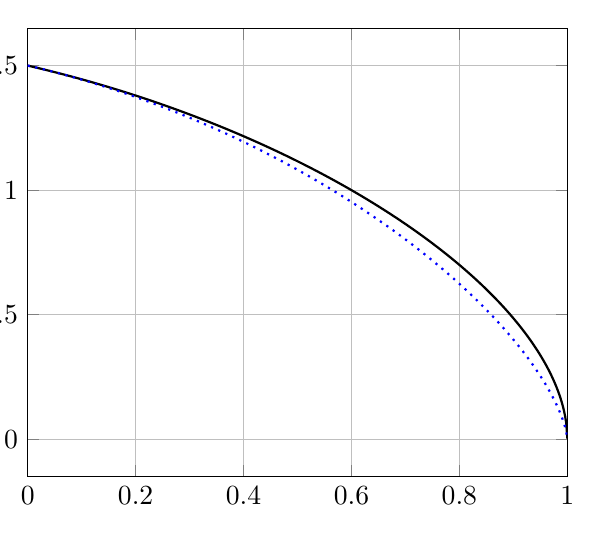
\begin{tikzpicture}[trim axis left,
    declare function={entropy(\x) = - \x * ln(\x)/ln(2) - (1 - \x) * ln(1 - \x) / ln(2); },
    declare function={gamma(\x) = (1 - x) / 2 + sqrt( 1 - x^2 ); },
    declare function={phi(\x) = (3/2) * (1 + x)^(1/3) * ( 1 - x )^(2/3); }
    %declare function = { entropy(\x) = 1; },
    ]
    \begin{axis}[domain=0:1,
      samples=500,
      enlarge x limits=false,
      grid=both,
      no markers]
      \addplot +[thick,black] { gamma(x) };
      \addplot +[thick,blue, dotted] { phi(x) };
    \end{axis}
  \end{tikzpicture}
  \qquad \qquad
  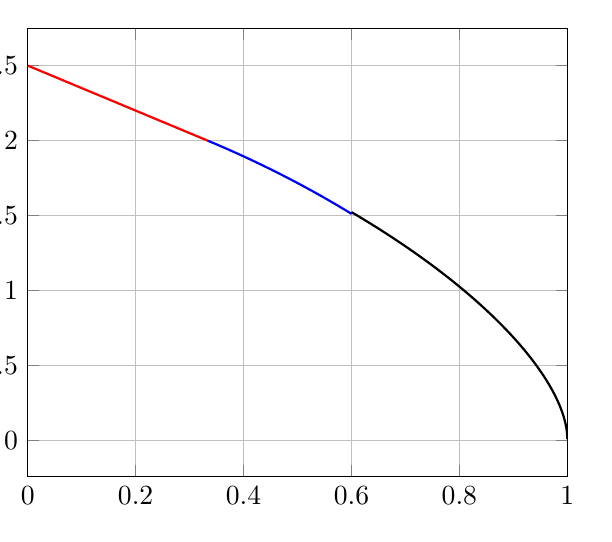
\begin{tikzpicture}[trim axis left,
    declare function={entropy(\x) = - \x * ln(\x)/ln(2) - (1 - \x) * ln(1 - \x) / ln(2); },
    declare function={gamma(\x) = (1 - x) / 2 + sqrt( 1 - x^2 ); },
    declare function={phi(\x) = (3/2) * (1 + x)^(1/3) * ( 1 - x )^(2/3); },
    declare function={psi(\x) = ( 1 - ln( (1+x)/(1-x) ) / ln(2) )^2 * ln(2) / 63; }
    %    declare function = { entropy(\x) = 1; },
    ]
    \begin{axis}[domain=0:1,
      samples=500,
      enlarge x limits=false,
      grid=both,
      no markers]
      \addplot +[thick,domain=0:(1/3),red] {(5 - 3 * x) / 2};
      \addplot +[thick,domain=(1/3):0.6,blue] {2^(2/3) * phi(x)};
      \addplot +[thick,domain=0.6:1,black] { 2^(2/3 + psi(x) ) * phi(x) )};
    \end{axis}
  \end{tikzpicture}
  
  \caption{\emph{(Left)} It is instructive to consider the base of the exponential part of the bounds on $\Exp[ g(W_{n-d+1}\cdots W_n) ]$. The solid curve is the $d$th root of the upper bound from Claim~\ref{claim:t2star-exact} and the dotted curve is the $d$th root of the lower bound from Claim~\ref{claim:t1star-exact}. We can see that beyond $\epsilon \geq 0.6$, the largest term in $\Exp[ g(W_{n-d+1}\cdots W_n) ]$ is $O(1)$. \emph{(Right)} We consider the same for $\Exp[ g(W_{n-d+1}\cdots W_n)^2 ]$. The curves depict the $d$th root of the upper bounds Claim~\ref{claim:t1star-variance-exact} and Claim~\ref{claim:t2star-variance-exact}. We can see that beyond $\epsilon \geq 0.81$, the largest term in $\Exp[ g(W_{n-d+1}\cdots W_n)^2 ]$ is $O(1)$.
  }
  \label{fig:grinding-power-mean}
\end{figure}

} % end iftoggle{drawfigs}

\iftoggle{drawfigs}{

\begin{figure}
  \centering
  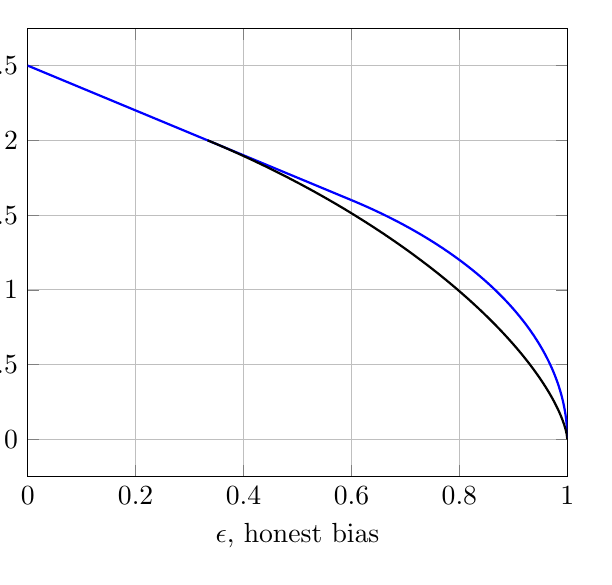
\begin{tikzpicture}[trim axis left,
    declare function={entropy(\x) = - \x * ln(\x)/ln(2) - (1 - \x) * ln(1 - \x) / ln(2); },
    %    declare function = { entropy(\x) = 1; },
    ]
    \begin{axis}[domain=0:1,
      samples=500,
      enlarge x limits=false,
      grid=both,
      xlabel={$\epsilon$, honest bias},
      no markers]
      \addplot +[thick,domain=0:(3/5),blue] {(5 - 3 * x)/2};
      \addplot +[thick,domain=(3/5):1,blue] {2 * sqrt( (1 - x^2))};
      % \addplot +[thick,domain=(3/5):1,red] {2 * sqrt( (1 - x^2))};
      \addplot +[thick,domain=(1/3):1,black] {(3/2^(1/3)) * (1+x)^(1/3) * (1-x)^(2/3)};
      % \addplot +[thick,domain=(3/5):1,black, dotted] {5/2 * (1 - x/2 - (6/25) * x^2 )};
      %\addplot +[thick,blue] { ((1-x)/2)^(2/3) * (1 + x)^(1/3) * 2^(entropy(x)) };

	  %\addplot +[thick,black] {(1-x)/2+sqrt(1 - x^2)};	
	  %\addplot +[thick,dotted,black] {(3/2)(1+x)^(1/3)(1-x)^(2/3)};	
    \end{axis}
  \end{tikzpicture}
  \caption{The blue curve is the $d$-th root of the bounds 
  from Proposition~\ref{prop:praos-moments-simple} and~\ref{prop:moments-t-large-eps}. 
  The black curve is the asymptotic bound from Claims~\ref{claim:t1star-variance-exact} and \ref{claim:t2star-variance-exact}.}
  \label{fig:grinding-power-variance}
\end{figure}

} % end iftoggle{drawfigs}


%=====================================================

